\section{Testprotokoll: Surge}
\label{sec:Test:Surge}
Wie in Kapitel \ref{sec:TestUndNorm} erwähnt, werden Surge-Tests zurchgeführt. Zur Auswahl stehen gemäss Kapitel \ref{sec:TestUndNorm} vier verschiedene Normprogramme. Es wurden das erste (Level 1) und das letzte (Level 4) Normprogramm durchgeführt, deren Ergebnisse werden nachfolgend dokumentiert. Der Testaufbau und die verwendeten Geräte werden in Kapitel \ref{sec:Testaufbau} erläutert.\\[0.25cm]
Die Auswirkungen der Tests wurden mit einem Oszilloskop gemessen. Nachfolgend werden die Abbildungen davon aufgezeigt und kurz erläutert.\\[0.5cm]
\begin{minipage}[b][10cm][t]{1\textwidth}
\centering
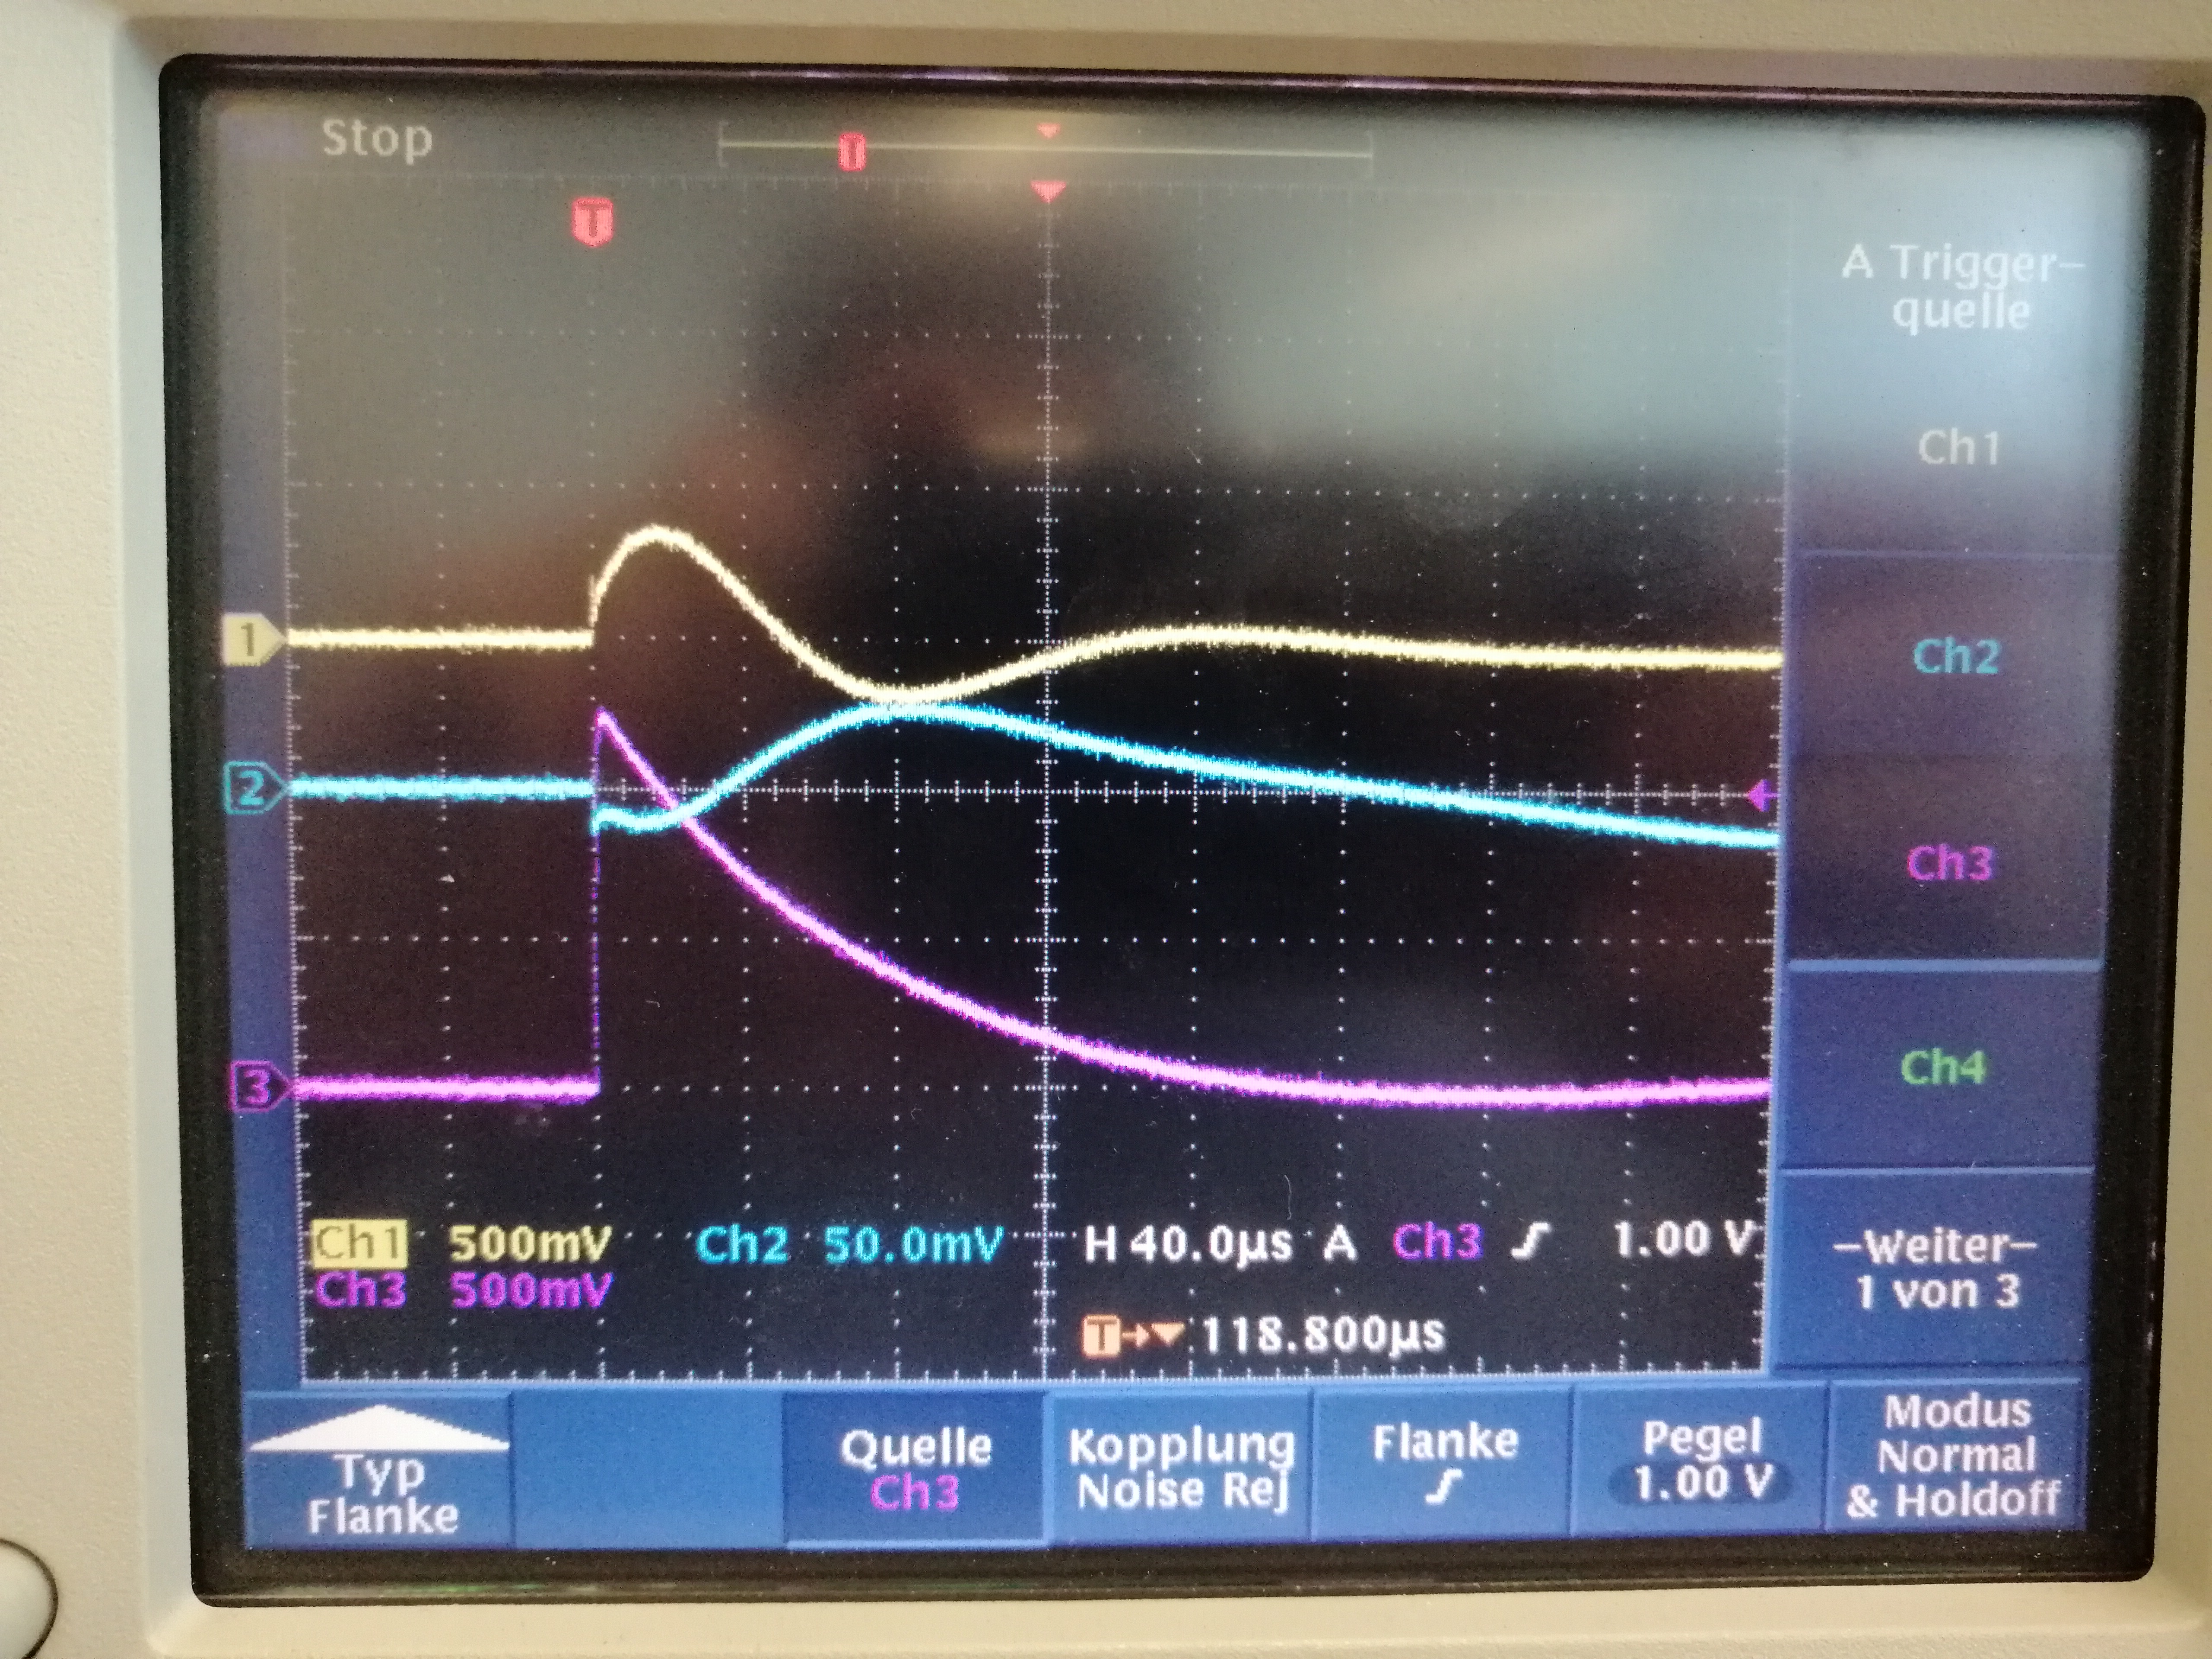
\includegraphics[angle=0,width=0.75\textwidth]{graphics/Surge1.jpg}
\captionof{figure}{Signalmessung während Surge-Test, Level 1, positive Polarität.}
\label{fig:Surge1}
\end{minipage}
Abbildung \ref{fig:Surge1} zeigt die verschiedenen Messsignale. Die Stossspannung des Surge-Tests (Lila) ist deutlich zu sehen mit einer steilen Flanke und einem Abklingen über 200$\mu$s. Der zur Stossspannung zugehöriger Strom (Blau) ist ebenfalls zu sehen mit einem kleinen, steilen Abfall, gefolgt von einer Erhöhung welche sich dann wieder senkt. Das Messsignal (Gelb) zeigt eine Überhöhung mit gefolgtem Einschwingen über ebenfalls etwa 200$\mu$s.\\[0.5cm]
\begin{minipage}[b][10cm][t]{1\textwidth}
\centering
\includegraphics[angle=0,width=0.75\textwidth]{graphics/Surge2.jpg}
\captionof{figure}{Signalmessung während Surge-Test, Level 1, negative Polarität.}
\label{fig:Surge2}
\end{minipage}
Abbildung \ref{fig:Surge2} zeigt das gespiegelte Verhalten von Abildung \ref{fig:Surge1}.\\[0.5cm]
\begin{minipage}[b][10cm][t]{1\textwidth}
\centering
\includegraphics[angle=0,width=0.75\textwidth]{graphics/Surge3.jpg}
\captionof{figure}{Signalmessung während Surge-Test, Level 4, positive Polarität.}
\label{fig:Surge3}
\end{minipage}
Abbildung \ref{fig:Surge3} zeigt die verschiedenen Messsignale. Die Stossspannung des Surge-Tests (Lila) ist deutlich zu sehen mit einer steilen Flanke und einem Abklingen über 240$\mu$s. Der zur Stossspannung zugehöriger Strom (Blau) ist ebenfalls zu sehen mit einem kleinen, steilen Abfall, gefolgt von einer Erhöhung welche sich dann wieder senkt. Das Messsignal (Gelb) zeigt eine Überhöhung mit gefolgtem Einschwingen über ebenfalls etwa 240$\mu$s.\\[0.5cm]
\begin{minipage}[b][10cm][t]{1\textwidth}
\centering
\includegraphics[angle=0,width=0.75\textwidth]{graphics/Surge4.jpg}
\captionof{figure}{Signalmessung während Surge-Test, Level 4, negative Polarität.}
\label{fig:Surge4}
\end{minipage}
Abbildung \ref{fig:Surge4} zeigt das gespiegelte Verhalten von Abildung \ref{fig:Surge3}.\\[0.5cm]
\begin{tabular}{|l|l|p{5cm}|p{5cm}|}
\hline 
\rule[-1ex]{0pt}{2.5ex} Prüfspannung & Prüflevel & Anzahl Surges pro Polarität & Auswirkung \\ 
\hline 
\rule[-1ex]{0pt}{2.5ex} 500 V & 1 & Bis mindestens 1 Surge mit dem Oszilloskop gut eingefangen werden konnte & Verlust der Messfähigkeit bei aktivem Surge. Wieder funktionsfähig unmittelbar nach dem Surge. \\ 
\hline 
\rule[-1ex]{0pt}{2.5ex} 4000 V & 4 & Bis mindestens 1 Surge mit dem Oszilloskop gut eingefangen werden konnte & Verlust der Messfähigkeit bei aktivem Surge. Wieder funktionsfähig unmittelbar nach dem Surge. \\ 
\hline 
\end{tabular} 
\captionof{table}{Prüfungsergebnis Surge-Tests.}
\label{tab:SurgeErgebnis}
\vspace*{0.25cm}
Tabelle \ref{tab:SurgeErgebnis} listet die Ergebnisse der durchgeführten Surge-Normprogramme auf. Es ist zu erkennen, dass bei jedem Surge-Test die gleichen Auswirkungen zu sehen waren. Die Gesamtauswertung der Tests wird in einem separaten Kapitel (Kapitel \ref{sec:Auswertung}) behandelt.\\
